\begin{figure}[H]
\centering
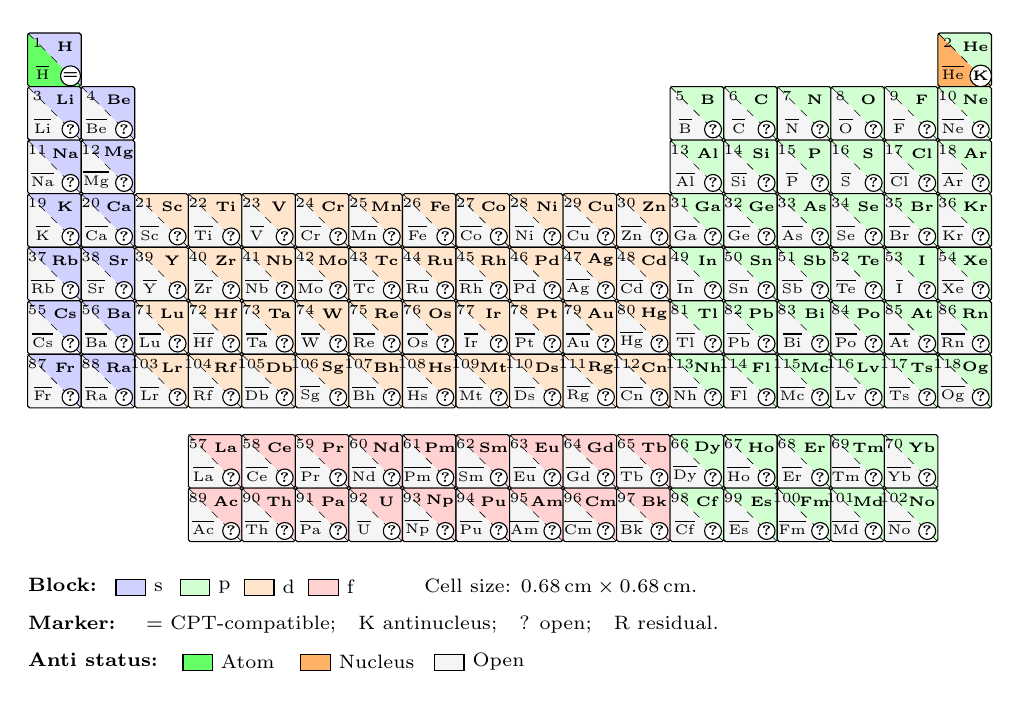
\begin{tikzpicture}[x=0.68cm, y=0.68cm, every node/.style={inner sep=0pt}]
\path[use as bounding box] (0,0.1) rectangle (18,-12.2);
\fill[blue!18, rounded corners=0.7pt] (0,0) -- (1,0) -- (1,-1) -- cycle;
\fill[green!60, rounded corners=0.7pt] (0,0) -- (0,-1) -- (1,-1) -- cycle;
\draw[black, rounded corners=0.7pt] (0,0) rectangle (1,-1);
\draw[black, dashed, very thin] (0,0) -- (1,-1);
\node at (0.7,-0.25) {\tiny \textbf{H}};
\node at (0.28,-0.73) {\tiny \textbf{$\overline{\mathrm{H}}$}};
\node at (0.18,-0.18) {\tiny 1};
\node[fill=white, draw=black, circle, inner sep=0.4pt] at (0.8,-0.8) {\tiny \textbf{=}};
\fill[green!18, rounded corners=0.7pt] (17,0) -- (18,0) -- (18,-1) -- cycle;
\fill[orange!60, rounded corners=0.7pt] (17,0) -- (17,-1) -- (18,-1) -- cycle;
\draw[black, rounded corners=0.7pt] (17,0) rectangle (18,-1);
\draw[black, dashed, very thin] (17,0) -- (18,-1);
\node at (17.7,-0.25) {\tiny \textbf{He}};
\node at (17.28,-0.73) {\tiny \textbf{$\overline{\mathrm{He}}$}};
\node at (17.18,-0.18) {\tiny 2};
\node[fill=white, draw=black, circle, inner sep=0.4pt] at (17.8,-0.8) {\tiny \textbf{K}};
\fill[blue!18, rounded corners=0.7pt] (0,-1) -- (1,-1) -- (1,-2) -- cycle;
\fill[gray!8, rounded corners=0.7pt] (0,-1) -- (0,-2) -- (1,-2) -- cycle;
\draw[black, rounded corners=0.7pt] (0,-1) rectangle (1,-2);
\draw[black, dashed, very thin] (0,-1) -- (1,-2);
\node at (0.7,-1.25) {\tiny \textbf{Li}};
\node at (0.28,-1.73) {\tiny \textbf{$\overline{\mathrm{Li}}$}};
\node at (0.18,-1.18) {\tiny 3};
\node[fill=white, draw=black, circle, inner sep=0.4pt] at (0.8,-1.8) {\tiny \textbf{?}};
\fill[blue!18, rounded corners=0.7pt] (1,-1) -- (2,-1) -- (2,-2) -- cycle;
\fill[gray!8, rounded corners=0.7pt] (1,-1) -- (1,-2) -- (2,-2) -- cycle;
\draw[black, rounded corners=0.7pt] (1,-1) rectangle (2,-2);
\draw[black, dashed, very thin] (1,-1) -- (2,-2);
\node at (1.7,-1.25) {\tiny \textbf{Be}};
\node at (1.28,-1.73) {\tiny \textbf{$\overline{\mathrm{Be}}$}};
\node at (1.18,-1.18) {\tiny 4};
\node[fill=white, draw=black, circle, inner sep=0.4pt] at (1.8,-1.8) {\tiny \textbf{?}};
\fill[green!18, rounded corners=0.7pt] (12,-1) -- (13,-1) -- (13,-2) -- cycle;
\fill[gray!8, rounded corners=0.7pt] (12,-1) -- (12,-2) -- (13,-2) -- cycle;
\draw[black, rounded corners=0.7pt] (12,-1) rectangle (13,-2);
\draw[black, dashed, very thin] (12,-1) -- (13,-2);
\node at (12.7,-1.25) {\tiny \textbf{B}};
\node at (12.28,-1.73) {\tiny \textbf{$\overline{\mathrm{B}}$}};
\node at (12.18,-1.18) {\tiny 5};
\node[fill=white, draw=black, circle, inner sep=0.4pt] at (12.8,-1.8) {\tiny \textbf{?}};
\fill[green!18, rounded corners=0.7pt] (13,-1) -- (14,-1) -- (14,-2) -- cycle;
\fill[gray!8, rounded corners=0.7pt] (13,-1) -- (13,-2) -- (14,-2) -- cycle;
\draw[black, rounded corners=0.7pt] (13,-1) rectangle (14,-2);
\draw[black, dashed, very thin] (13,-1) -- (14,-2);
\node at (13.7,-1.25) {\tiny \textbf{C}};
\node at (13.28,-1.73) {\tiny \textbf{$\overline{\mathrm{C}}$}};
\node at (13.18,-1.18) {\tiny 6};
\node[fill=white, draw=black, circle, inner sep=0.4pt] at (13.8,-1.8) {\tiny \textbf{?}};
\fill[green!18, rounded corners=0.7pt] (14,-1) -- (15,-1) -- (15,-2) -- cycle;
\fill[gray!8, rounded corners=0.7pt] (14,-1) -- (14,-2) -- (15,-2) -- cycle;
\draw[black, rounded corners=0.7pt] (14,-1) rectangle (15,-2);
\draw[black, dashed, very thin] (14,-1) -- (15,-2);
\node at (14.7,-1.25) {\tiny \textbf{N}};
\node at (14.28,-1.73) {\tiny \textbf{$\overline{\mathrm{N}}$}};
\node at (14.18,-1.18) {\tiny 7};
\node[fill=white, draw=black, circle, inner sep=0.4pt] at (14.8,-1.8) {\tiny \textbf{?}};
\fill[green!18, rounded corners=0.7pt] (15,-1) -- (16,-1) -- (16,-2) -- cycle;
\fill[gray!8, rounded corners=0.7pt] (15,-1) -- (15,-2) -- (16,-2) -- cycle;
\draw[black, rounded corners=0.7pt] (15,-1) rectangle (16,-2);
\draw[black, dashed, very thin] (15,-1) -- (16,-2);
\node at (15.7,-1.25) {\tiny \textbf{O}};
\node at (15.28,-1.73) {\tiny \textbf{$\overline{\mathrm{O}}$}};
\node at (15.18,-1.18) {\tiny 8};
\node[fill=white, draw=black, circle, inner sep=0.4pt] at (15.8,-1.8) {\tiny \textbf{?}};
\fill[green!18, rounded corners=0.7pt] (16,-1) -- (17,-1) -- (17,-2) -- cycle;
\fill[gray!8, rounded corners=0.7pt] (16,-1) -- (16,-2) -- (17,-2) -- cycle;
\draw[black, rounded corners=0.7pt] (16,-1) rectangle (17,-2);
\draw[black, dashed, very thin] (16,-1) -- (17,-2);
\node at (16.7,-1.25) {\tiny \textbf{F}};
\node at (16.28,-1.73) {\tiny \textbf{$\overline{\mathrm{F}}$}};
\node at (16.18,-1.18) {\tiny 9};
\node[fill=white, draw=black, circle, inner sep=0.4pt] at (16.8,-1.8) {\tiny \textbf{?}};
\fill[green!18, rounded corners=0.7pt] (17,-1) -- (18,-1) -- (18,-2) -- cycle;
\fill[gray!8, rounded corners=0.7pt] (17,-1) -- (17,-2) -- (18,-2) -- cycle;
\draw[black, rounded corners=0.7pt] (17,-1) rectangle (18,-2);
\draw[black, dashed, very thin] (17,-1) -- (18,-2);
\node at (17.7,-1.25) {\tiny \textbf{Ne}};
\node at (17.28,-1.73) {\tiny \textbf{$\overline{\mathrm{Ne}}$}};
\node at (17.18,-1.18) {\tiny 10};
\node[fill=white, draw=black, circle, inner sep=0.4pt] at (17.8,-1.8) {\tiny \textbf{?}};
\fill[blue!18, rounded corners=0.7pt] (0,-2) -- (1,-2) -- (1,-3) -- cycle;
\fill[gray!8, rounded corners=0.7pt] (0,-2) -- (0,-3) -- (1,-3) -- cycle;
\draw[black, rounded corners=0.7pt] (0,-2) rectangle (1,-3);
\draw[black, dashed, very thin] (0,-2) -- (1,-3);
\node at (0.7,-2.25) {\tiny \textbf{Na}};
\node at (0.28,-2.73) {\tiny \textbf{$\overline{\mathrm{Na}}$}};
\node at (0.18,-2.18) {\tiny 11};
\node[fill=white, draw=black, circle, inner sep=0.4pt] at (0.8,-2.8) {\tiny \textbf{?}};
\fill[blue!18, rounded corners=0.7pt] (1,-2) -- (2,-2) -- (2,-3) -- cycle;
\fill[gray!8, rounded corners=0.7pt] (1,-2) -- (1,-3) -- (2,-3) -- cycle;
\draw[black, rounded corners=0.7pt] (1,-2) rectangle (2,-3);
\draw[black, dashed, very thin] (1,-2) -- (2,-3);
\node at (1.7,-2.25) {\tiny \textbf{Mg}};
\node at (1.28,-2.73) {\tiny \textbf{$\overline{\mathrm{Mg}}$}};
\node at (1.18,-2.18) {\tiny 12};
\node[fill=white, draw=black, circle, inner sep=0.4pt] at (1.8,-2.8) {\tiny \textbf{?}};
\fill[green!18, rounded corners=0.7pt] (12,-2) -- (13,-2) -- (13,-3) -- cycle;
\fill[gray!8, rounded corners=0.7pt] (12,-2) -- (12,-3) -- (13,-3) -- cycle;
\draw[black, rounded corners=0.7pt] (12,-2) rectangle (13,-3);
\draw[black, dashed, very thin] (12,-2) -- (13,-3);
\node at (12.7,-2.25) {\tiny \textbf{Al}};
\node at (12.28,-2.73) {\tiny \textbf{$\overline{\mathrm{Al}}$}};
\node at (12.18,-2.18) {\tiny 13};
\node[fill=white, draw=black, circle, inner sep=0.4pt] at (12.8,-2.8) {\tiny \textbf{?}};
\fill[green!18, rounded corners=0.7pt] (13,-2) -- (14,-2) -- (14,-3) -- cycle;
\fill[gray!8, rounded corners=0.7pt] (13,-2) -- (13,-3) -- (14,-3) -- cycle;
\draw[black, rounded corners=0.7pt] (13,-2) rectangle (14,-3);
\draw[black, dashed, very thin] (13,-2) -- (14,-3);
\node at (13.7,-2.25) {\tiny \textbf{Si}};
\node at (13.28,-2.73) {\tiny \textbf{$\overline{\mathrm{Si}}$}};
\node at (13.18,-2.18) {\tiny 14};
\node[fill=white, draw=black, circle, inner sep=0.4pt] at (13.8,-2.8) {\tiny \textbf{?}};
\fill[green!18, rounded corners=0.7pt] (14,-2) -- (15,-2) -- (15,-3) -- cycle;
\fill[gray!8, rounded corners=0.7pt] (14,-2) -- (14,-3) -- (15,-3) -- cycle;
\draw[black, rounded corners=0.7pt] (14,-2) rectangle (15,-3);
\draw[black, dashed, very thin] (14,-2) -- (15,-3);
\node at (14.7,-2.25) {\tiny \textbf{P}};
\node at (14.28,-2.73) {\tiny \textbf{$\overline{\mathrm{P}}$}};
\node at (14.18,-2.18) {\tiny 15};
\node[fill=white, draw=black, circle, inner sep=0.4pt] at (14.8,-2.8) {\tiny \textbf{?}};
\fill[green!18, rounded corners=0.7pt] (15,-2) -- (16,-2) -- (16,-3) -- cycle;
\fill[gray!8, rounded corners=0.7pt] (15,-2) -- (15,-3) -- (16,-3) -- cycle;
\draw[black, rounded corners=0.7pt] (15,-2) rectangle (16,-3);
\draw[black, dashed, very thin] (15,-2) -- (16,-3);
\node at (15.7,-2.25) {\tiny \textbf{S}};
\node at (15.28,-2.73) {\tiny \textbf{$\overline{\mathrm{S}}$}};
\node at (15.18,-2.18) {\tiny 16};
\node[fill=white, draw=black, circle, inner sep=0.4pt] at (15.8,-2.8) {\tiny \textbf{?}};
\fill[green!18, rounded corners=0.7pt] (16,-2) -- (17,-2) -- (17,-3) -- cycle;
\fill[gray!8, rounded corners=0.7pt] (16,-2) -- (16,-3) -- (17,-3) -- cycle;
\draw[black, rounded corners=0.7pt] (16,-2) rectangle (17,-3);
\draw[black, dashed, very thin] (16,-2) -- (17,-3);
\node at (16.7,-2.25) {\tiny \textbf{Cl}};
\node at (16.28,-2.73) {\tiny \textbf{$\overline{\mathrm{Cl}}$}};
\node at (16.18,-2.18) {\tiny 17};
\node[fill=white, draw=black, circle, inner sep=0.4pt] at (16.8,-2.8) {\tiny \textbf{?}};
\fill[green!18, rounded corners=0.7pt] (17,-2) -- (18,-2) -- (18,-3) -- cycle;
\fill[gray!8, rounded corners=0.7pt] (17,-2) -- (17,-3) -- (18,-3) -- cycle;
\draw[black, rounded corners=0.7pt] (17,-2) rectangle (18,-3);
\draw[black, dashed, very thin] (17,-2) -- (18,-3);
\node at (17.7,-2.25) {\tiny \textbf{Ar}};
\node at (17.28,-2.73) {\tiny \textbf{$\overline{\mathrm{Ar}}$}};
\node at (17.18,-2.18) {\tiny 18};
\node[fill=white, draw=black, circle, inner sep=0.4pt] at (17.8,-2.8) {\tiny \textbf{?}};
\fill[blue!18, rounded corners=0.7pt] (0,-3) -- (1,-3) -- (1,-4) -- cycle;
\fill[gray!8, rounded corners=0.7pt] (0,-3) -- (0,-4) -- (1,-4) -- cycle;
\draw[black, rounded corners=0.7pt] (0,-3) rectangle (1,-4);
\draw[black, dashed, very thin] (0,-3) -- (1,-4);
\node at (0.7,-3.25) {\tiny \textbf{K}};
\node at (0.28,-3.73) {\tiny \textbf{$\overline{\mathrm{K}}$}};
\node at (0.18,-3.18) {\tiny 19};
\node[fill=white, draw=black, circle, inner sep=0.4pt] at (0.8,-3.8) {\tiny \textbf{?}};
\fill[blue!18, rounded corners=0.7pt] (1,-3) -- (2,-3) -- (2,-4) -- cycle;
\fill[gray!8, rounded corners=0.7pt] (1,-3) -- (1,-4) -- (2,-4) -- cycle;
\draw[black, rounded corners=0.7pt] (1,-3) rectangle (2,-4);
\draw[black, dashed, very thin] (1,-3) -- (2,-4);
\node at (1.7,-3.25) {\tiny \textbf{Ca}};
\node at (1.28,-3.73) {\tiny \textbf{$\overline{\mathrm{Ca}}$}};
\node at (1.18,-3.18) {\tiny 20};
\node[fill=white, draw=black, circle, inner sep=0.4pt] at (1.8,-3.8) {\tiny \textbf{?}};
\fill[orange!20, rounded corners=0.7pt] (2,-3) -- (3,-3) -- (3,-4) -- cycle;
\fill[gray!8, rounded corners=0.7pt] (2,-3) -- (2,-4) -- (3,-4) -- cycle;
\draw[black, rounded corners=0.7pt] (2,-3) rectangle (3,-4);
\draw[black, dashed, very thin] (2,-3) -- (3,-4);
\node at (2.7,-3.25) {\tiny \textbf{Sc}};
\node at (2.2800000000000002,-3.73) {\tiny \textbf{$\overline{\mathrm{Sc}}$}};
\node at (2.18,-3.18) {\tiny 21};
\node[fill=white, draw=black, circle, inner sep=0.4pt] at (2.8,-3.8) {\tiny \textbf{?}};
\fill[orange!20, rounded corners=0.7pt] (3,-3) -- (4,-3) -- (4,-4) -- cycle;
\fill[gray!8, rounded corners=0.7pt] (3,-3) -- (3,-4) -- (4,-4) -- cycle;
\draw[black, rounded corners=0.7pt] (3,-3) rectangle (4,-4);
\draw[black, dashed, very thin] (3,-3) -- (4,-4);
\node at (3.7,-3.25) {\tiny \textbf{Ti}};
\node at (3.2800000000000002,-3.73) {\tiny \textbf{$\overline{\mathrm{Ti}}$}};
\node at (3.18,-3.18) {\tiny 22};
\node[fill=white, draw=black, circle, inner sep=0.4pt] at (3.8,-3.8) {\tiny \textbf{?}};
\fill[orange!20, rounded corners=0.7pt] (4,-3) -- (5,-3) -- (5,-4) -- cycle;
\fill[gray!8, rounded corners=0.7pt] (4,-3) -- (4,-4) -- (5,-4) -- cycle;
\draw[black, rounded corners=0.7pt] (4,-3) rectangle (5,-4);
\draw[black, dashed, very thin] (4,-3) -- (5,-4);
\node at (4.7,-3.25) {\tiny \textbf{V}};
\node at (4.28,-3.73) {\tiny \textbf{$\overline{\mathrm{V}}$}};
\node at (4.18,-3.18) {\tiny 23};
\node[fill=white, draw=black, circle, inner sep=0.4pt] at (4.8,-3.8) {\tiny \textbf{?}};
\fill[orange!20, rounded corners=0.7pt] (5,-3) -- (6,-3) -- (6,-4) -- cycle;
\fill[gray!8, rounded corners=0.7pt] (5,-3) -- (5,-4) -- (6,-4) -- cycle;
\draw[black, rounded corners=0.7pt] (5,-3) rectangle (6,-4);
\draw[black, dashed, very thin] (5,-3) -- (6,-4);
\node at (5.7,-3.25) {\tiny \textbf{Cr}};
\node at (5.28,-3.73) {\tiny \textbf{$\overline{\mathrm{Cr}}$}};
\node at (5.18,-3.18) {\tiny 24};
\node[fill=white, draw=black, circle, inner sep=0.4pt] at (5.8,-3.8) {\tiny \textbf{?}};
\fill[orange!20, rounded corners=0.7pt] (6,-3) -- (7,-3) -- (7,-4) -- cycle;
\fill[gray!8, rounded corners=0.7pt] (6,-3) -- (6,-4) -- (7,-4) -- cycle;
\draw[black, rounded corners=0.7pt] (6,-3) rectangle (7,-4);
\draw[black, dashed, very thin] (6,-3) -- (7,-4);
\node at (6.7,-3.25) {\tiny \textbf{Mn}};
\node at (6.28,-3.73) {\tiny \textbf{$\overline{\mathrm{Mn}}$}};
\node at (6.18,-3.18) {\tiny 25};
\node[fill=white, draw=black, circle, inner sep=0.4pt] at (6.8,-3.8) {\tiny \textbf{?}};
\fill[orange!20, rounded corners=0.7pt] (7,-3) -- (8,-3) -- (8,-4) -- cycle;
\fill[gray!8, rounded corners=0.7pt] (7,-3) -- (7,-4) -- (8,-4) -- cycle;
\draw[black, rounded corners=0.7pt] (7,-3) rectangle (8,-4);
\draw[black, dashed, very thin] (7,-3) -- (8,-4);
\node at (7.7,-3.25) {\tiny \textbf{Fe}};
\node at (7.28,-3.73) {\tiny \textbf{$\overline{\mathrm{Fe}}$}};
\node at (7.18,-3.18) {\tiny 26};
\node[fill=white, draw=black, circle, inner sep=0.4pt] at (7.8,-3.8) {\tiny \textbf{?}};
\fill[orange!20, rounded corners=0.7pt] (8,-3) -- (9,-3) -- (9,-4) -- cycle;
\fill[gray!8, rounded corners=0.7pt] (8,-3) -- (8,-4) -- (9,-4) -- cycle;
\draw[black, rounded corners=0.7pt] (8,-3) rectangle (9,-4);
\draw[black, dashed, very thin] (8,-3) -- (9,-4);
\node at (8.7,-3.25) {\tiny \textbf{Co}};
\node at (8.28,-3.73) {\tiny \textbf{$\overline{\mathrm{Co}}$}};
\node at (8.18,-3.18) {\tiny 27};
\node[fill=white, draw=black, circle, inner sep=0.4pt] at (8.8,-3.8) {\tiny \textbf{?}};
\fill[orange!20, rounded corners=0.7pt] (9,-3) -- (10,-3) -- (10,-4) -- cycle;
\fill[gray!8, rounded corners=0.7pt] (9,-3) -- (9,-4) -- (10,-4) -- cycle;
\draw[black, rounded corners=0.7pt] (9,-3) rectangle (10,-4);
\draw[black, dashed, very thin] (9,-3) -- (10,-4);
\node at (9.7,-3.25) {\tiny \textbf{Ni}};
\node at (9.28,-3.73) {\tiny \textbf{$\overline{\mathrm{Ni}}$}};
\node at (9.18,-3.18) {\tiny 28};
\node[fill=white, draw=black, circle, inner sep=0.4pt] at (9.8,-3.8) {\tiny \textbf{?}};
\fill[orange!20, rounded corners=0.7pt] (10,-3) -- (11,-3) -- (11,-4) -- cycle;
\fill[gray!8, rounded corners=0.7pt] (10,-3) -- (10,-4) -- (11,-4) -- cycle;
\draw[black, rounded corners=0.7pt] (10,-3) rectangle (11,-4);
\draw[black, dashed, very thin] (10,-3) -- (11,-4);
\node at (10.7,-3.25) {\tiny \textbf{Cu}};
\node at (10.28,-3.73) {\tiny \textbf{$\overline{\mathrm{Cu}}$}};
\node at (10.18,-3.18) {\tiny 29};
\node[fill=white, draw=black, circle, inner sep=0.4pt] at (10.8,-3.8) {\tiny \textbf{?}};
\fill[orange!20, rounded corners=0.7pt] (11,-3) -- (12,-3) -- (12,-4) -- cycle;
\fill[gray!8, rounded corners=0.7pt] (11,-3) -- (11,-4) -- (12,-4) -- cycle;
\draw[black, rounded corners=0.7pt] (11,-3) rectangle (12,-4);
\draw[black, dashed, very thin] (11,-3) -- (12,-4);
\node at (11.7,-3.25) {\tiny \textbf{Zn}};
\node at (11.28,-3.73) {\tiny \textbf{$\overline{\mathrm{Zn}}$}};
\node at (11.18,-3.18) {\tiny 30};
\node[fill=white, draw=black, circle, inner sep=0.4pt] at (11.8,-3.8) {\tiny \textbf{?}};
\fill[green!18, rounded corners=0.7pt] (12,-3) -- (13,-3) -- (13,-4) -- cycle;
\fill[gray!8, rounded corners=0.7pt] (12,-3) -- (12,-4) -- (13,-4) -- cycle;
\draw[black, rounded corners=0.7pt] (12,-3) rectangle (13,-4);
\draw[black, dashed, very thin] (12,-3) -- (13,-4);
\node at (12.7,-3.25) {\tiny \textbf{Ga}};
\node at (12.28,-3.73) {\tiny \textbf{$\overline{\mathrm{Ga}}$}};
\node at (12.18,-3.18) {\tiny 31};
\node[fill=white, draw=black, circle, inner sep=0.4pt] at (12.8,-3.8) {\tiny \textbf{?}};
\fill[green!18, rounded corners=0.7pt] (13,-3) -- (14,-3) -- (14,-4) -- cycle;
\fill[gray!8, rounded corners=0.7pt] (13,-3) -- (13,-4) -- (14,-4) -- cycle;
\draw[black, rounded corners=0.7pt] (13,-3) rectangle (14,-4);
\draw[black, dashed, very thin] (13,-3) -- (14,-4);
\node at (13.7,-3.25) {\tiny \textbf{Ge}};
\node at (13.28,-3.73) {\tiny \textbf{$\overline{\mathrm{Ge}}$}};
\node at (13.18,-3.18) {\tiny 32};
\node[fill=white, draw=black, circle, inner sep=0.4pt] at (13.8,-3.8) {\tiny \textbf{?}};
\fill[green!18, rounded corners=0.7pt] (14,-3) -- (15,-3) -- (15,-4) -- cycle;
\fill[gray!8, rounded corners=0.7pt] (14,-3) -- (14,-4) -- (15,-4) -- cycle;
\draw[black, rounded corners=0.7pt] (14,-3) rectangle (15,-4);
\draw[black, dashed, very thin] (14,-3) -- (15,-4);
\node at (14.7,-3.25) {\tiny \textbf{As}};
\node at (14.28,-3.73) {\tiny \textbf{$\overline{\mathrm{As}}$}};
\node at (14.18,-3.18) {\tiny 33};
\node[fill=white, draw=black, circle, inner sep=0.4pt] at (14.8,-3.8) {\tiny \textbf{?}};
\fill[green!18, rounded corners=0.7pt] (15,-3) -- (16,-3) -- (16,-4) -- cycle;
\fill[gray!8, rounded corners=0.7pt] (15,-3) -- (15,-4) -- (16,-4) -- cycle;
\draw[black, rounded corners=0.7pt] (15,-3) rectangle (16,-4);
\draw[black, dashed, very thin] (15,-3) -- (16,-4);
\node at (15.7,-3.25) {\tiny \textbf{Se}};
\node at (15.28,-3.73) {\tiny \textbf{$\overline{\mathrm{Se}}$}};
\node at (15.18,-3.18) {\tiny 34};
\node[fill=white, draw=black, circle, inner sep=0.4pt] at (15.8,-3.8) {\tiny \textbf{?}};
\fill[green!18, rounded corners=0.7pt] (16,-3) -- (17,-3) -- (17,-4) -- cycle;
\fill[gray!8, rounded corners=0.7pt] (16,-3) -- (16,-4) -- (17,-4) -- cycle;
\draw[black, rounded corners=0.7pt] (16,-3) rectangle (17,-4);
\draw[black, dashed, very thin] (16,-3) -- (17,-4);
\node at (16.7,-3.25) {\tiny \textbf{Br}};
\node at (16.28,-3.73) {\tiny \textbf{$\overline{\mathrm{Br}}$}};
\node at (16.18,-3.18) {\tiny 35};
\node[fill=white, draw=black, circle, inner sep=0.4pt] at (16.8,-3.8) {\tiny \textbf{?}};
\fill[green!18, rounded corners=0.7pt] (17,-3) -- (18,-3) -- (18,-4) -- cycle;
\fill[gray!8, rounded corners=0.7pt] (17,-3) -- (17,-4) -- (18,-4) -- cycle;
\draw[black, rounded corners=0.7pt] (17,-3) rectangle (18,-4);
\draw[black, dashed, very thin] (17,-3) -- (18,-4);
\node at (17.7,-3.25) {\tiny \textbf{Kr}};
\node at (17.28,-3.73) {\tiny \textbf{$\overline{\mathrm{Kr}}$}};
\node at (17.18,-3.18) {\tiny 36};
\node[fill=white, draw=black, circle, inner sep=0.4pt] at (17.8,-3.8) {\tiny \textbf{?}};
\fill[blue!18, rounded corners=0.7pt] (0,-4) -- (1,-4) -- (1,-5) -- cycle;
\fill[gray!8, rounded corners=0.7pt] (0,-4) -- (0,-5) -- (1,-5) -- cycle;
\draw[black, rounded corners=0.7pt] (0,-4) rectangle (1,-5);
\draw[black, dashed, very thin] (0,-4) -- (1,-5);
\node at (0.7,-4.25) {\tiny \textbf{Rb}};
\node at (0.28,-4.73) {\tiny \textbf{$\overline{\mathrm{Rb}}$}};
\node at (0.18,-4.18) {\tiny 37};
\node[fill=white, draw=black, circle, inner sep=0.4pt] at (0.8,-4.8) {\tiny \textbf{?}};
\fill[blue!18, rounded corners=0.7pt] (1,-4) -- (2,-4) -- (2,-5) -- cycle;
\fill[gray!8, rounded corners=0.7pt] (1,-4) -- (1,-5) -- (2,-5) -- cycle;
\draw[black, rounded corners=0.7pt] (1,-4) rectangle (2,-5);
\draw[black, dashed, very thin] (1,-4) -- (2,-5);
\node at (1.7,-4.25) {\tiny \textbf{Sr}};
\node at (1.28,-4.73) {\tiny \textbf{$\overline{\mathrm{Sr}}$}};
\node at (1.18,-4.18) {\tiny 38};
\node[fill=white, draw=black, circle, inner sep=0.4pt] at (1.8,-4.8) {\tiny \textbf{?}};
\fill[orange!20, rounded corners=0.7pt] (2,-4) -- (3,-4) -- (3,-5) -- cycle;
\fill[gray!8, rounded corners=0.7pt] (2,-4) -- (2,-5) -- (3,-5) -- cycle;
\draw[black, rounded corners=0.7pt] (2,-4) rectangle (3,-5);
\draw[black, dashed, very thin] (2,-4) -- (3,-5);
\node at (2.7,-4.25) {\tiny \textbf{Y}};
\node at (2.2800000000000002,-4.73) {\tiny \textbf{$\overline{\mathrm{Y}}$}};
\node at (2.18,-4.18) {\tiny 39};
\node[fill=white, draw=black, circle, inner sep=0.4pt] at (2.8,-4.8) {\tiny \textbf{?}};
\fill[orange!20, rounded corners=0.7pt] (3,-4) -- (4,-4) -- (4,-5) -- cycle;
\fill[gray!8, rounded corners=0.7pt] (3,-4) -- (3,-5) -- (4,-5) -- cycle;
\draw[black, rounded corners=0.7pt] (3,-4) rectangle (4,-5);
\draw[black, dashed, very thin] (3,-4) -- (4,-5);
\node at (3.7,-4.25) {\tiny \textbf{Zr}};
\node at (3.2800000000000002,-4.73) {\tiny \textbf{$\overline{\mathrm{Zr}}$}};
\node at (3.18,-4.18) {\tiny 40};
\node[fill=white, draw=black, circle, inner sep=0.4pt] at (3.8,-4.8) {\tiny \textbf{?}};
\fill[orange!20, rounded corners=0.7pt] (4,-4) -- (5,-4) -- (5,-5) -- cycle;
\fill[gray!8, rounded corners=0.7pt] (4,-4) -- (4,-5) -- (5,-5) -- cycle;
\draw[black, rounded corners=0.7pt] (4,-4) rectangle (5,-5);
\draw[black, dashed, very thin] (4,-4) -- (5,-5);
\node at (4.7,-4.25) {\tiny \textbf{Nb}};
\node at (4.28,-4.73) {\tiny \textbf{$\overline{\mathrm{Nb}}$}};
\node at (4.18,-4.18) {\tiny 41};
\node[fill=white, draw=black, circle, inner sep=0.4pt] at (4.8,-4.8) {\tiny \textbf{?}};
\fill[orange!20, rounded corners=0.7pt] (5,-4) -- (6,-4) -- (6,-5) -- cycle;
\fill[gray!8, rounded corners=0.7pt] (5,-4) -- (5,-5) -- (6,-5) -- cycle;
\draw[black, rounded corners=0.7pt] (5,-4) rectangle (6,-5);
\draw[black, dashed, very thin] (5,-4) -- (6,-5);
\node at (5.7,-4.25) {\tiny \textbf{Mo}};
\node at (5.28,-4.73) {\tiny \textbf{$\overline{\mathrm{Mo}}$}};
\node at (5.18,-4.18) {\tiny 42};
\node[fill=white, draw=black, circle, inner sep=0.4pt] at (5.8,-4.8) {\tiny \textbf{?}};
\fill[orange!20, rounded corners=0.7pt] (6,-4) -- (7,-4) -- (7,-5) -- cycle;
\fill[gray!8, rounded corners=0.7pt] (6,-4) -- (6,-5) -- (7,-5) -- cycle;
\draw[black, rounded corners=0.7pt] (6,-4) rectangle (7,-5);
\draw[black, dashed, very thin] (6,-4) -- (7,-5);
\node at (6.7,-4.25) {\tiny \textbf{Tc}};
\node at (6.28,-4.73) {\tiny \textbf{$\overline{\mathrm{Tc}}$}};
\node at (6.18,-4.18) {\tiny 43};
\node[fill=white, draw=black, circle, inner sep=0.4pt] at (6.8,-4.8) {\tiny \textbf{?}};
\fill[orange!20, rounded corners=0.7pt] (7,-4) -- (8,-4) -- (8,-5) -- cycle;
\fill[gray!8, rounded corners=0.7pt] (7,-4) -- (7,-5) -- (8,-5) -- cycle;
\draw[black, rounded corners=0.7pt] (7,-4) rectangle (8,-5);
\draw[black, dashed, very thin] (7,-4) -- (8,-5);
\node at (7.7,-4.25) {\tiny \textbf{Ru}};
\node at (7.28,-4.73) {\tiny \textbf{$\overline{\mathrm{Ru}}$}};
\node at (7.18,-4.18) {\tiny 44};
\node[fill=white, draw=black, circle, inner sep=0.4pt] at (7.8,-4.8) {\tiny \textbf{?}};
\fill[orange!20, rounded corners=0.7pt] (8,-4) -- (9,-4) -- (9,-5) -- cycle;
\fill[gray!8, rounded corners=0.7pt] (8,-4) -- (8,-5) -- (9,-5) -- cycle;
\draw[black, rounded corners=0.7pt] (8,-4) rectangle (9,-5);
\draw[black, dashed, very thin] (8,-4) -- (9,-5);
\node at (8.7,-4.25) {\tiny \textbf{Rh}};
\node at (8.28,-4.73) {\tiny \textbf{$\overline{\mathrm{Rh}}$}};
\node at (8.18,-4.18) {\tiny 45};
\node[fill=white, draw=black, circle, inner sep=0.4pt] at (8.8,-4.8) {\tiny \textbf{?}};
\fill[orange!20, rounded corners=0.7pt] (9,-4) -- (10,-4) -- (10,-5) -- cycle;
\fill[gray!8, rounded corners=0.7pt] (9,-4) -- (9,-5) -- (10,-5) -- cycle;
\draw[black, rounded corners=0.7pt] (9,-4) rectangle (10,-5);
\draw[black, dashed, very thin] (9,-4) -- (10,-5);
\node at (9.7,-4.25) {\tiny \textbf{Pd}};
\node at (9.28,-4.73) {\tiny \textbf{$\overline{\mathrm{Pd}}$}};
\node at (9.18,-4.18) {\tiny 46};
\node[fill=white, draw=black, circle, inner sep=0.4pt] at (9.8,-4.8) {\tiny \textbf{?}};
\fill[orange!20, rounded corners=0.7pt] (10,-4) -- (11,-4) -- (11,-5) -- cycle;
\fill[gray!8, rounded corners=0.7pt] (10,-4) -- (10,-5) -- (11,-5) -- cycle;
\draw[black, rounded corners=0.7pt] (10,-4) rectangle (11,-5);
\draw[black, dashed, very thin] (10,-4) -- (11,-5);
\node at (10.7,-4.25) {\tiny \textbf{Ag}};
\node at (10.28,-4.73) {\tiny \textbf{$\overline{\mathrm{Ag}}$}};
\node at (10.18,-4.18) {\tiny 47};
\node[fill=white, draw=black, circle, inner sep=0.4pt] at (10.8,-4.8) {\tiny \textbf{?}};
\fill[orange!20, rounded corners=0.7pt] (11,-4) -- (12,-4) -- (12,-5) -- cycle;
\fill[gray!8, rounded corners=0.7pt] (11,-4) -- (11,-5) -- (12,-5) -- cycle;
\draw[black, rounded corners=0.7pt] (11,-4) rectangle (12,-5);
\draw[black, dashed, very thin] (11,-4) -- (12,-5);
\node at (11.7,-4.25) {\tiny \textbf{Cd}};
\node at (11.28,-4.73) {\tiny \textbf{$\overline{\mathrm{Cd}}$}};
\node at (11.18,-4.18) {\tiny 48};
\node[fill=white, draw=black, circle, inner sep=0.4pt] at (11.8,-4.8) {\tiny \textbf{?}};
\fill[green!18, rounded corners=0.7pt] (12,-4) -- (13,-4) -- (13,-5) -- cycle;
\fill[gray!8, rounded corners=0.7pt] (12,-4) -- (12,-5) -- (13,-5) -- cycle;
\draw[black, rounded corners=0.7pt] (12,-4) rectangle (13,-5);
\draw[black, dashed, very thin] (12,-4) -- (13,-5);
\node at (12.7,-4.25) {\tiny \textbf{In}};
\node at (12.28,-4.73) {\tiny \textbf{$\overline{\mathrm{In}}$}};
\node at (12.18,-4.18) {\tiny 49};
\node[fill=white, draw=black, circle, inner sep=0.4pt] at (12.8,-4.8) {\tiny \textbf{?}};
\fill[green!18, rounded corners=0.7pt] (13,-4) -- (14,-4) -- (14,-5) -- cycle;
\fill[gray!8, rounded corners=0.7pt] (13,-4) -- (13,-5) -- (14,-5) -- cycle;
\draw[black, rounded corners=0.7pt] (13,-4) rectangle (14,-5);
\draw[black, dashed, very thin] (13,-4) -- (14,-5);
\node at (13.7,-4.25) {\tiny \textbf{Sn}};
\node at (13.28,-4.73) {\tiny \textbf{$\overline{\mathrm{Sn}}$}};
\node at (13.18,-4.18) {\tiny 50};
\node[fill=white, draw=black, circle, inner sep=0.4pt] at (13.8,-4.8) {\tiny \textbf{?}};
\fill[green!18, rounded corners=0.7pt] (14,-4) -- (15,-4) -- (15,-5) -- cycle;
\fill[gray!8, rounded corners=0.7pt] (14,-4) -- (14,-5) -- (15,-5) -- cycle;
\draw[black, rounded corners=0.7pt] (14,-4) rectangle (15,-5);
\draw[black, dashed, very thin] (14,-4) -- (15,-5);
\node at (14.7,-4.25) {\tiny \textbf{Sb}};
\node at (14.28,-4.73) {\tiny \textbf{$\overline{\mathrm{Sb}}$}};
\node at (14.18,-4.18) {\tiny 51};
\node[fill=white, draw=black, circle, inner sep=0.4pt] at (14.8,-4.8) {\tiny \textbf{?}};
\fill[green!18, rounded corners=0.7pt] (15,-4) -- (16,-4) -- (16,-5) -- cycle;
\fill[gray!8, rounded corners=0.7pt] (15,-4) -- (15,-5) -- (16,-5) -- cycle;
\draw[black, rounded corners=0.7pt] (15,-4) rectangle (16,-5);
\draw[black, dashed, very thin] (15,-4) -- (16,-5);
\node at (15.7,-4.25) {\tiny \textbf{Te}};
\node at (15.28,-4.73) {\tiny \textbf{$\overline{\mathrm{Te}}$}};
\node at (15.18,-4.18) {\tiny 52};
\node[fill=white, draw=black, circle, inner sep=0.4pt] at (15.8,-4.8) {\tiny \textbf{?}};
\fill[green!18, rounded corners=0.7pt] (16,-4) -- (17,-4) -- (17,-5) -- cycle;
\fill[gray!8, rounded corners=0.7pt] (16,-4) -- (16,-5) -- (17,-5) -- cycle;
\draw[black, rounded corners=0.7pt] (16,-4) rectangle (17,-5);
\draw[black, dashed, very thin] (16,-4) -- (17,-5);
\node at (16.7,-4.25) {\tiny \textbf{I}};
\node at (16.28,-4.73) {\tiny \textbf{$\overline{\mathrm{I}}$}};
\node at (16.18,-4.18) {\tiny 53};
\node[fill=white, draw=black, circle, inner sep=0.4pt] at (16.8,-4.8) {\tiny \textbf{?}};
\fill[green!18, rounded corners=0.7pt] (17,-4) -- (18,-4) -- (18,-5) -- cycle;
\fill[gray!8, rounded corners=0.7pt] (17,-4) -- (17,-5) -- (18,-5) -- cycle;
\draw[black, rounded corners=0.7pt] (17,-4) rectangle (18,-5);
\draw[black, dashed, very thin] (17,-4) -- (18,-5);
\node at (17.7,-4.25) {\tiny \textbf{Xe}};
\node at (17.28,-4.73) {\tiny \textbf{$\overline{\mathrm{Xe}}$}};
\node at (17.18,-4.18) {\tiny 54};
\node[fill=white, draw=black, circle, inner sep=0.4pt] at (17.8,-4.8) {\tiny \textbf{?}};
\fill[blue!18, rounded corners=0.7pt] (0,-5) -- (1,-5) -- (1,-6) -- cycle;
\fill[gray!8, rounded corners=0.7pt] (0,-5) -- (0,-6) -- (1,-6) -- cycle;
\draw[black, rounded corners=0.7pt] (0,-5) rectangle (1,-6);
\draw[black, dashed, very thin] (0,-5) -- (1,-6);
\node at (0.7,-5.25) {\tiny \textbf{Cs}};
\node at (0.28,-5.73) {\tiny \textbf{$\overline{\mathrm{Cs}}$}};
\node at (0.18,-5.18) {\tiny 55};
\node[fill=white, draw=black, circle, inner sep=0.4pt] at (0.8,-5.8) {\tiny \textbf{?}};
\fill[blue!18, rounded corners=0.7pt] (1,-5) -- (2,-5) -- (2,-6) -- cycle;
\fill[gray!8, rounded corners=0.7pt] (1,-5) -- (1,-6) -- (2,-6) -- cycle;
\draw[black, rounded corners=0.7pt] (1,-5) rectangle (2,-6);
\draw[black, dashed, very thin] (1,-5) -- (2,-6);
\node at (1.7,-5.25) {\tiny \textbf{Ba}};
\node at (1.28,-5.73) {\tiny \textbf{$\overline{\mathrm{Ba}}$}};
\node at (1.18,-5.18) {\tiny 56};
\node[fill=white, draw=black, circle, inner sep=0.4pt] at (1.8,-5.8) {\tiny \textbf{?}};
\fill[orange!20, rounded corners=0.7pt] (2,-5) -- (3,-5) -- (3,-6) -- cycle;
\fill[gray!8, rounded corners=0.7pt] (2,-5) -- (2,-6) -- (3,-6) -- cycle;
\draw[black, rounded corners=0.7pt] (2,-5) rectangle (3,-6);
\draw[black, dashed, very thin] (2,-5) -- (3,-6);
\node at (2.7,-5.25) {\tiny \textbf{Lu}};
\node at (2.2800000000000002,-5.73) {\tiny \textbf{$\overline{\mathrm{Lu}}$}};
\node at (2.18,-5.18) {\tiny 71};
\node[fill=white, draw=black, circle, inner sep=0.4pt] at (2.8,-5.8) {\tiny \textbf{?}};
\fill[orange!20, rounded corners=0.7pt] (3,-5) -- (4,-5) -- (4,-6) -- cycle;
\fill[gray!8, rounded corners=0.7pt] (3,-5) -- (3,-6) -- (4,-6) -- cycle;
\draw[black, rounded corners=0.7pt] (3,-5) rectangle (4,-6);
\draw[black, dashed, very thin] (3,-5) -- (4,-6);
\node at (3.7,-5.25) {\tiny \textbf{Hf}};
\node at (3.2800000000000002,-5.73) {\tiny \textbf{$\overline{\mathrm{Hf}}$}};
\node at (3.18,-5.18) {\tiny 72};
\node[fill=white, draw=black, circle, inner sep=0.4pt] at (3.8,-5.8) {\tiny \textbf{?}};
\fill[orange!20, rounded corners=0.7pt] (4,-5) -- (5,-5) -- (5,-6) -- cycle;
\fill[gray!8, rounded corners=0.7pt] (4,-5) -- (4,-6) -- (5,-6) -- cycle;
\draw[black, rounded corners=0.7pt] (4,-5) rectangle (5,-6);
\draw[black, dashed, very thin] (4,-5) -- (5,-6);
\node at (4.7,-5.25) {\tiny \textbf{Ta}};
\node at (4.28,-5.73) {\tiny \textbf{$\overline{\mathrm{Ta}}$}};
\node at (4.18,-5.18) {\tiny 73};
\node[fill=white, draw=black, circle, inner sep=0.4pt] at (4.8,-5.8) {\tiny \textbf{?}};
\fill[orange!20, rounded corners=0.7pt] (5,-5) -- (6,-5) -- (6,-6) -- cycle;
\fill[gray!8, rounded corners=0.7pt] (5,-5) -- (5,-6) -- (6,-6) -- cycle;
\draw[black, rounded corners=0.7pt] (5,-5) rectangle (6,-6);
\draw[black, dashed, very thin] (5,-5) -- (6,-6);
\node at (5.7,-5.25) {\tiny \textbf{W}};
\node at (5.28,-5.73) {\tiny \textbf{$\overline{\mathrm{W}}$}};
\node at (5.18,-5.18) {\tiny 74};
\node[fill=white, draw=black, circle, inner sep=0.4pt] at (5.8,-5.8) {\tiny \textbf{?}};
\fill[orange!20, rounded corners=0.7pt] (6,-5) -- (7,-5) -- (7,-6) -- cycle;
\fill[gray!8, rounded corners=0.7pt] (6,-5) -- (6,-6) -- (7,-6) -- cycle;
\draw[black, rounded corners=0.7pt] (6,-5) rectangle (7,-6);
\draw[black, dashed, very thin] (6,-5) -- (7,-6);
\node at (6.7,-5.25) {\tiny \textbf{Re}};
\node at (6.28,-5.73) {\tiny \textbf{$\overline{\mathrm{Re}}$}};
\node at (6.18,-5.18) {\tiny 75};
\node[fill=white, draw=black, circle, inner sep=0.4pt] at (6.8,-5.8) {\tiny \textbf{?}};
\fill[orange!20, rounded corners=0.7pt] (7,-5) -- (8,-5) -- (8,-6) -- cycle;
\fill[gray!8, rounded corners=0.7pt] (7,-5) -- (7,-6) -- (8,-6) -- cycle;
\draw[black, rounded corners=0.7pt] (7,-5) rectangle (8,-6);
\draw[black, dashed, very thin] (7,-5) -- (8,-6);
\node at (7.7,-5.25) {\tiny \textbf{Os}};
\node at (7.28,-5.73) {\tiny \textbf{$\overline{\mathrm{Os}}$}};
\node at (7.18,-5.18) {\tiny 76};
\node[fill=white, draw=black, circle, inner sep=0.4pt] at (7.8,-5.8) {\tiny \textbf{?}};
\fill[orange!20, rounded corners=0.7pt] (8,-5) -- (9,-5) -- (9,-6) -- cycle;
\fill[gray!8, rounded corners=0.7pt] (8,-5) -- (8,-6) -- (9,-6) -- cycle;
\draw[black, rounded corners=0.7pt] (8,-5) rectangle (9,-6);
\draw[black, dashed, very thin] (8,-5) -- (9,-6);
\node at (8.7,-5.25) {\tiny \textbf{Ir}};
\node at (8.28,-5.73) {\tiny \textbf{$\overline{\mathrm{Ir}}$}};
\node at (8.18,-5.18) {\tiny 77};
\node[fill=white, draw=black, circle, inner sep=0.4pt] at (8.8,-5.8) {\tiny \textbf{?}};
\fill[orange!20, rounded corners=0.7pt] (9,-5) -- (10,-5) -- (10,-6) -- cycle;
\fill[gray!8, rounded corners=0.7pt] (9,-5) -- (9,-6) -- (10,-6) -- cycle;
\draw[black, rounded corners=0.7pt] (9,-5) rectangle (10,-6);
\draw[black, dashed, very thin] (9,-5) -- (10,-6);
\node at (9.7,-5.25) {\tiny \textbf{Pt}};
\node at (9.28,-5.73) {\tiny \textbf{$\overline{\mathrm{Pt}}$}};
\node at (9.18,-5.18) {\tiny 78};
\node[fill=white, draw=black, circle, inner sep=0.4pt] at (9.8,-5.8) {\tiny \textbf{?}};
\fill[orange!20, rounded corners=0.7pt] (10,-5) -- (11,-5) -- (11,-6) -- cycle;
\fill[gray!8, rounded corners=0.7pt] (10,-5) -- (10,-6) -- (11,-6) -- cycle;
\draw[black, rounded corners=0.7pt] (10,-5) rectangle (11,-6);
\draw[black, dashed, very thin] (10,-5) -- (11,-6);
\node at (10.7,-5.25) {\tiny \textbf{Au}};
\node at (10.28,-5.73) {\tiny \textbf{$\overline{\mathrm{Au}}$}};
\node at (10.18,-5.18) {\tiny 79};
\node[fill=white, draw=black, circle, inner sep=0.4pt] at (10.8,-5.8) {\tiny \textbf{?}};
\fill[orange!20, rounded corners=0.7pt] (11,-5) -- (12,-5) -- (12,-6) -- cycle;
\fill[gray!8, rounded corners=0.7pt] (11,-5) -- (11,-6) -- (12,-6) -- cycle;
\draw[black, rounded corners=0.7pt] (11,-5) rectangle (12,-6);
\draw[black, dashed, very thin] (11,-5) -- (12,-6);
\node at (11.7,-5.25) {\tiny \textbf{Hg}};
\node at (11.28,-5.73) {\tiny \textbf{$\overline{\mathrm{Hg}}$}};
\node at (11.18,-5.18) {\tiny 80};
\node[fill=white, draw=black, circle, inner sep=0.4pt] at (11.8,-5.8) {\tiny \textbf{?}};
\fill[green!18, rounded corners=0.7pt] (12,-5) -- (13,-5) -- (13,-6) -- cycle;
\fill[gray!8, rounded corners=0.7pt] (12,-5) -- (12,-6) -- (13,-6) -- cycle;
\draw[black, rounded corners=0.7pt] (12,-5) rectangle (13,-6);
\draw[black, dashed, very thin] (12,-5) -- (13,-6);
\node at (12.7,-5.25) {\tiny \textbf{Tl}};
\node at (12.28,-5.73) {\tiny \textbf{$\overline{\mathrm{Tl}}$}};
\node at (12.18,-5.18) {\tiny 81};
\node[fill=white, draw=black, circle, inner sep=0.4pt] at (12.8,-5.8) {\tiny \textbf{?}};
\fill[green!18, rounded corners=0.7pt] (13,-5) -- (14,-5) -- (14,-6) -- cycle;
\fill[gray!8, rounded corners=0.7pt] (13,-5) -- (13,-6) -- (14,-6) -- cycle;
\draw[black, rounded corners=0.7pt] (13,-5) rectangle (14,-6);
\draw[black, dashed, very thin] (13,-5) -- (14,-6);
\node at (13.7,-5.25) {\tiny \textbf{Pb}};
\node at (13.28,-5.73) {\tiny \textbf{$\overline{\mathrm{Pb}}$}};
\node at (13.18,-5.18) {\tiny 82};
\node[fill=white, draw=black, circle, inner sep=0.4pt] at (13.8,-5.8) {\tiny \textbf{?}};
\fill[green!18, rounded corners=0.7pt] (14,-5) -- (15,-5) -- (15,-6) -- cycle;
\fill[gray!8, rounded corners=0.7pt] (14,-5) -- (14,-6) -- (15,-6) -- cycle;
\draw[black, rounded corners=0.7pt] (14,-5) rectangle (15,-6);
\draw[black, dashed, very thin] (14,-5) -- (15,-6);
\node at (14.7,-5.25) {\tiny \textbf{Bi}};
\node at (14.28,-5.73) {\tiny \textbf{$\overline{\mathrm{Bi}}$}};
\node at (14.18,-5.18) {\tiny 83};
\node[fill=white, draw=black, circle, inner sep=0.4pt] at (14.8,-5.8) {\tiny \textbf{?}};
\fill[green!18, rounded corners=0.7pt] (15,-5) -- (16,-5) -- (16,-6) -- cycle;
\fill[gray!8, rounded corners=0.7pt] (15,-5) -- (15,-6) -- (16,-6) -- cycle;
\draw[black, rounded corners=0.7pt] (15,-5) rectangle (16,-6);
\draw[black, dashed, very thin] (15,-5) -- (16,-6);
\node at (15.7,-5.25) {\tiny \textbf{Po}};
\node at (15.28,-5.73) {\tiny \textbf{$\overline{\mathrm{Po}}$}};
\node at (15.18,-5.18) {\tiny 84};
\node[fill=white, draw=black, circle, inner sep=0.4pt] at (15.8,-5.8) {\tiny \textbf{?}};
\fill[green!18, rounded corners=0.7pt] (16,-5) -- (17,-5) -- (17,-6) -- cycle;
\fill[gray!8, rounded corners=0.7pt] (16,-5) -- (16,-6) -- (17,-6) -- cycle;
\draw[black, rounded corners=0.7pt] (16,-5) rectangle (17,-6);
\draw[black, dashed, very thin] (16,-5) -- (17,-6);
\node at (16.7,-5.25) {\tiny \textbf{At}};
\node at (16.28,-5.73) {\tiny \textbf{$\overline{\mathrm{At}}$}};
\node at (16.18,-5.18) {\tiny 85};
\node[fill=white, draw=black, circle, inner sep=0.4pt] at (16.8,-5.8) {\tiny \textbf{?}};
\fill[green!18, rounded corners=0.7pt] (17,-5) -- (18,-5) -- (18,-6) -- cycle;
\fill[gray!8, rounded corners=0.7pt] (17,-5) -- (17,-6) -- (18,-6) -- cycle;
\draw[black, rounded corners=0.7pt] (17,-5) rectangle (18,-6);
\draw[black, dashed, very thin] (17,-5) -- (18,-6);
\node at (17.7,-5.25) {\tiny \textbf{Rn}};
\node at (17.28,-5.73) {\tiny \textbf{$\overline{\mathrm{Rn}}$}};
\node at (17.18,-5.18) {\tiny 86};
\node[fill=white, draw=black, circle, inner sep=0.4pt] at (17.8,-5.8) {\tiny \textbf{?}};
\fill[blue!18, rounded corners=0.7pt] (0,-6) -- (1,-6) -- (1,-7) -- cycle;
\fill[gray!8, rounded corners=0.7pt] (0,-6) -- (0,-7) -- (1,-7) -- cycle;
\draw[black, rounded corners=0.7pt] (0,-6) rectangle (1,-7);
\draw[black, dashed, very thin] (0,-6) -- (1,-7);
\node at (0.7,-6.25) {\tiny \textbf{Fr}};
\node at (0.28,-6.73) {\tiny \textbf{$\overline{\mathrm{Fr}}$}};
\node at (0.18,-6.18) {\tiny 87};
\node[fill=white, draw=black, circle, inner sep=0.4pt] at (0.8,-6.8) {\tiny \textbf{?}};
\fill[blue!18, rounded corners=0.7pt] (1,-6) -- (2,-6) -- (2,-7) -- cycle;
\fill[gray!8, rounded corners=0.7pt] (1,-6) -- (1,-7) -- (2,-7) -- cycle;
\draw[black, rounded corners=0.7pt] (1,-6) rectangle (2,-7);
\draw[black, dashed, very thin] (1,-6) -- (2,-7);
\node at (1.7,-6.25) {\tiny \textbf{Ra}};
\node at (1.28,-6.73) {\tiny \textbf{$\overline{\mathrm{Ra}}$}};
\node at (1.18,-6.18) {\tiny 88};
\node[fill=white, draw=black, circle, inner sep=0.4pt] at (1.8,-6.8) {\tiny \textbf{?}};
\fill[orange!20, rounded corners=0.7pt] (2,-6) -- (3,-6) -- (3,-7) -- cycle;
\fill[gray!8, rounded corners=0.7pt] (2,-6) -- (2,-7) -- (3,-7) -- cycle;
\draw[black, rounded corners=0.7pt] (2,-6) rectangle (3,-7);
\draw[black, dashed, very thin] (2,-6) -- (3,-7);
\node at (2.7,-6.25) {\tiny \textbf{Lr}};
\node at (2.2800000000000002,-6.73) {\tiny \textbf{$\overline{\mathrm{Lr}}$}};
\node at (2.18,-6.18) {\tiny 103};
\node[fill=white, draw=black, circle, inner sep=0.4pt] at (2.8,-6.8) {\tiny \textbf{?}};
\fill[orange!20, rounded corners=0.7pt] (3,-6) -- (4,-6) -- (4,-7) -- cycle;
\fill[gray!8, rounded corners=0.7pt] (3,-6) -- (3,-7) -- (4,-7) -- cycle;
\draw[black, rounded corners=0.7pt] (3,-6) rectangle (4,-7);
\draw[black, dashed, very thin] (3,-6) -- (4,-7);
\node at (3.7,-6.25) {\tiny \textbf{Rf}};
\node at (3.2800000000000002,-6.73) {\tiny \textbf{$\overline{\mathrm{Rf}}$}};
\node at (3.18,-6.18) {\tiny 104};
\node[fill=white, draw=black, circle, inner sep=0.4pt] at (3.8,-6.8) {\tiny \textbf{?}};
\fill[orange!20, rounded corners=0.7pt] (4,-6) -- (5,-6) -- (5,-7) -- cycle;
\fill[gray!8, rounded corners=0.7pt] (4,-6) -- (4,-7) -- (5,-7) -- cycle;
\draw[black, rounded corners=0.7pt] (4,-6) rectangle (5,-7);
\draw[black, dashed, very thin] (4,-6) -- (5,-7);
\node at (4.7,-6.25) {\tiny \textbf{Db}};
\node at (4.28,-6.73) {\tiny \textbf{$\overline{\mathrm{Db}}$}};
\node at (4.18,-6.18) {\tiny 105};
\node[fill=white, draw=black, circle, inner sep=0.4pt] at (4.8,-6.8) {\tiny \textbf{?}};
\fill[orange!20, rounded corners=0.7pt] (5,-6) -- (6,-6) -- (6,-7) -- cycle;
\fill[gray!8, rounded corners=0.7pt] (5,-6) -- (5,-7) -- (6,-7) -- cycle;
\draw[black, rounded corners=0.7pt] (5,-6) rectangle (6,-7);
\draw[black, dashed, very thin] (5,-6) -- (6,-7);
\node at (5.7,-6.25) {\tiny \textbf{Sg}};
\node at (5.28,-6.73) {\tiny \textbf{$\overline{\mathrm{Sg}}$}};
\node at (5.18,-6.18) {\tiny 106};
\node[fill=white, draw=black, circle, inner sep=0.4pt] at (5.8,-6.8) {\tiny \textbf{?}};
\fill[orange!20, rounded corners=0.7pt] (6,-6) -- (7,-6) -- (7,-7) -- cycle;
\fill[gray!8, rounded corners=0.7pt] (6,-6) -- (6,-7) -- (7,-7) -- cycle;
\draw[black, rounded corners=0.7pt] (6,-6) rectangle (7,-7);
\draw[black, dashed, very thin] (6,-6) -- (7,-7);
\node at (6.7,-6.25) {\tiny \textbf{Bh}};
\node at (6.28,-6.73) {\tiny \textbf{$\overline{\mathrm{Bh}}$}};
\node at (6.18,-6.18) {\tiny 107};
\node[fill=white, draw=black, circle, inner sep=0.4pt] at (6.8,-6.8) {\tiny \textbf{?}};
\fill[orange!20, rounded corners=0.7pt] (7,-6) -- (8,-6) -- (8,-7) -- cycle;
\fill[gray!8, rounded corners=0.7pt] (7,-6) -- (7,-7) -- (8,-7) -- cycle;
\draw[black, rounded corners=0.7pt] (7,-6) rectangle (8,-7);
\draw[black, dashed, very thin] (7,-6) -- (8,-7);
\node at (7.7,-6.25) {\tiny \textbf{Hs}};
\node at (7.28,-6.73) {\tiny \textbf{$\overline{\mathrm{Hs}}$}};
\node at (7.18,-6.18) {\tiny 108};
\node[fill=white, draw=black, circle, inner sep=0.4pt] at (7.8,-6.8) {\tiny \textbf{?}};
\fill[orange!20, rounded corners=0.7pt] (8,-6) -- (9,-6) -- (9,-7) -- cycle;
\fill[gray!8, rounded corners=0.7pt] (8,-6) -- (8,-7) -- (9,-7) -- cycle;
\draw[black, rounded corners=0.7pt] (8,-6) rectangle (9,-7);
\draw[black, dashed, very thin] (8,-6) -- (9,-7);
\node at (8.7,-6.25) {\tiny \textbf{Mt}};
\node at (8.28,-6.73) {\tiny \textbf{$\overline{\mathrm{Mt}}$}};
\node at (8.18,-6.18) {\tiny 109};
\node[fill=white, draw=black, circle, inner sep=0.4pt] at (8.8,-6.8) {\tiny \textbf{?}};
\fill[orange!20, rounded corners=0.7pt] (9,-6) -- (10,-6) -- (10,-7) -- cycle;
\fill[gray!8, rounded corners=0.7pt] (9,-6) -- (9,-7) -- (10,-7) -- cycle;
\draw[black, rounded corners=0.7pt] (9,-6) rectangle (10,-7);
\draw[black, dashed, very thin] (9,-6) -- (10,-7);
\node at (9.7,-6.25) {\tiny \textbf{Ds}};
\node at (9.28,-6.73) {\tiny \textbf{$\overline{\mathrm{Ds}}$}};
\node at (9.18,-6.18) {\tiny 110};
\node[fill=white, draw=black, circle, inner sep=0.4pt] at (9.8,-6.8) {\tiny \textbf{?}};
\fill[orange!20, rounded corners=0.7pt] (10,-6) -- (11,-6) -- (11,-7) -- cycle;
\fill[gray!8, rounded corners=0.7pt] (10,-6) -- (10,-7) -- (11,-7) -- cycle;
\draw[black, rounded corners=0.7pt] (10,-6) rectangle (11,-7);
\draw[black, dashed, very thin] (10,-6) -- (11,-7);
\node at (10.7,-6.25) {\tiny \textbf{Rg}};
\node at (10.28,-6.73) {\tiny \textbf{$\overline{\mathrm{Rg}}$}};
\node at (10.18,-6.18) {\tiny 111};
\node[fill=white, draw=black, circle, inner sep=0.4pt] at (10.8,-6.8) {\tiny \textbf{?}};
\fill[orange!20, rounded corners=0.7pt] (11,-6) -- (12,-6) -- (12,-7) -- cycle;
\fill[gray!8, rounded corners=0.7pt] (11,-6) -- (11,-7) -- (12,-7) -- cycle;
\draw[black, rounded corners=0.7pt] (11,-6) rectangle (12,-7);
\draw[black, dashed, very thin] (11,-6) -- (12,-7);
\node at (11.7,-6.25) {\tiny \textbf{Cn}};
\node at (11.28,-6.73) {\tiny \textbf{$\overline{\mathrm{Cn}}$}};
\node at (11.18,-6.18) {\tiny 112};
\node[fill=white, draw=black, circle, inner sep=0.4pt] at (11.8,-6.8) {\tiny \textbf{?}};
\fill[green!18, rounded corners=0.7pt] (12,-6) -- (13,-6) -- (13,-7) -- cycle;
\fill[gray!8, rounded corners=0.7pt] (12,-6) -- (12,-7) -- (13,-7) -- cycle;
\draw[black, rounded corners=0.7pt] (12,-6) rectangle (13,-7);
\draw[black, dashed, very thin] (12,-6) -- (13,-7);
\node at (12.7,-6.25) {\tiny \textbf{Nh}};
\node at (12.28,-6.73) {\tiny \textbf{$\overline{\mathrm{Nh}}$}};
\node at (12.18,-6.18) {\tiny 113};
\node[fill=white, draw=black, circle, inner sep=0.4pt] at (12.8,-6.8) {\tiny \textbf{?}};
\fill[green!18, rounded corners=0.7pt] (13,-6) -- (14,-6) -- (14,-7) -- cycle;
\fill[gray!8, rounded corners=0.7pt] (13,-6) -- (13,-7) -- (14,-7) -- cycle;
\draw[black, rounded corners=0.7pt] (13,-6) rectangle (14,-7);
\draw[black, dashed, very thin] (13,-6) -- (14,-7);
\node at (13.7,-6.25) {\tiny \textbf{Fl}};
\node at (13.28,-6.73) {\tiny \textbf{$\overline{\mathrm{Fl}}$}};
\node at (13.18,-6.18) {\tiny 114};
\node[fill=white, draw=black, circle, inner sep=0.4pt] at (13.8,-6.8) {\tiny \textbf{?}};
\fill[green!18, rounded corners=0.7pt] (14,-6) -- (15,-6) -- (15,-7) -- cycle;
\fill[gray!8, rounded corners=0.7pt] (14,-6) -- (14,-7) -- (15,-7) -- cycle;
\draw[black, rounded corners=0.7pt] (14,-6) rectangle (15,-7);
\draw[black, dashed, very thin] (14,-6) -- (15,-7);
\node at (14.7,-6.25) {\tiny \textbf{Mc}};
\node at (14.28,-6.73) {\tiny \textbf{$\overline{\mathrm{Mc}}$}};
\node at (14.18,-6.18) {\tiny 115};
\node[fill=white, draw=black, circle, inner sep=0.4pt] at (14.8,-6.8) {\tiny \textbf{?}};
\fill[green!18, rounded corners=0.7pt] (15,-6) -- (16,-6) -- (16,-7) -- cycle;
\fill[gray!8, rounded corners=0.7pt] (15,-6) -- (15,-7) -- (16,-7) -- cycle;
\draw[black, rounded corners=0.7pt] (15,-6) rectangle (16,-7);
\draw[black, dashed, very thin] (15,-6) -- (16,-7);
\node at (15.7,-6.25) {\tiny \textbf{Lv}};
\node at (15.28,-6.73) {\tiny \textbf{$\overline{\mathrm{Lv}}$}};
\node at (15.18,-6.18) {\tiny 116};
\node[fill=white, draw=black, circle, inner sep=0.4pt] at (15.8,-6.8) {\tiny \textbf{?}};
\fill[green!18, rounded corners=0.7pt] (16,-6) -- (17,-6) -- (17,-7) -- cycle;
\fill[gray!8, rounded corners=0.7pt] (16,-6) -- (16,-7) -- (17,-7) -- cycle;
\draw[black, rounded corners=0.7pt] (16,-6) rectangle (17,-7);
\draw[black, dashed, very thin] (16,-6) -- (17,-7);
\node at (16.7,-6.25) {\tiny \textbf{Ts}};
\node at (16.28,-6.73) {\tiny \textbf{$\overline{\mathrm{Ts}}$}};
\node at (16.18,-6.18) {\tiny 117};
\node[fill=white, draw=black, circle, inner sep=0.4pt] at (16.8,-6.8) {\tiny \textbf{?}};
\fill[green!18, rounded corners=0.7pt] (17,-6) -- (18,-6) -- (18,-7) -- cycle;
\fill[gray!8, rounded corners=0.7pt] (17,-6) -- (17,-7) -- (18,-7) -- cycle;
\draw[black, rounded corners=0.7pt] (17,-6) rectangle (18,-7);
\draw[black, dashed, very thin] (17,-6) -- (18,-7);
\node at (17.7,-6.25) {\tiny \textbf{Og}};
\node at (17.28,-6.73) {\tiny \textbf{$\overline{\mathrm{Og}}$}};
\node at (17.18,-6.18) {\tiny 118};
\node[fill=white, draw=black, circle, inner sep=0.4pt] at (17.8,-6.8) {\tiny \textbf{?}};
\fill[red!18, rounded corners=0.7pt] (3,-7.5) -- (4,-7.5) -- (4,-8.5) -- cycle;
\fill[gray!8, rounded corners=0.7pt] (3,-7.5) -- (3,-8.5) -- (4,-8.5) -- cycle;
\draw[black, rounded corners=0.7pt] (3,-7.5) rectangle (4,-8.5);
\draw[black, dashed, very thin] (3,-7.5) -- (4,-8.5);
\node at (3.7,-7.75) {\tiny \textbf{La}};
\node at (3.2800000000000002,-8.23) {\tiny \textbf{$\overline{\mathrm{La}}$}};
\node at (3.18,-7.68) {\tiny 57};
\node[fill=white, draw=black, circle, inner sep=0.4pt] at (3.8,-8.3) {\tiny \textbf{?}};
\fill[red!18, rounded corners=0.7pt] (4,-7.5) -- (5,-7.5) -- (5,-8.5) -- cycle;
\fill[gray!8, rounded corners=0.7pt] (4,-7.5) -- (4,-8.5) -- (5,-8.5) -- cycle;
\draw[black, rounded corners=0.7pt] (4,-7.5) rectangle (5,-8.5);
\draw[black, dashed, very thin] (4,-7.5) -- (5,-8.5);
\node at (4.7,-7.75) {\tiny \textbf{Ce}};
\node at (4.28,-8.23) {\tiny \textbf{$\overline{\mathrm{Ce}}$}};
\node at (4.18,-7.68) {\tiny 58};
\node[fill=white, draw=black, circle, inner sep=0.4pt] at (4.8,-8.3) {\tiny \textbf{?}};
\fill[red!18, rounded corners=0.7pt] (5,-7.5) -- (6,-7.5) -- (6,-8.5) -- cycle;
\fill[gray!8, rounded corners=0.7pt] (5,-7.5) -- (5,-8.5) -- (6,-8.5) -- cycle;
\draw[black, rounded corners=0.7pt] (5,-7.5) rectangle (6,-8.5);
\draw[black, dashed, very thin] (5,-7.5) -- (6,-8.5);
\node at (5.7,-7.75) {\tiny \textbf{Pr}};
\node at (5.28,-8.23) {\tiny \textbf{$\overline{\mathrm{Pr}}$}};
\node at (5.18,-7.68) {\tiny 59};
\node[fill=white, draw=black, circle, inner sep=0.4pt] at (5.8,-8.3) {\tiny \textbf{?}};
\fill[red!18, rounded corners=0.7pt] (6,-7.5) -- (7,-7.5) -- (7,-8.5) -- cycle;
\fill[gray!8, rounded corners=0.7pt] (6,-7.5) -- (6,-8.5) -- (7,-8.5) -- cycle;
\draw[black, rounded corners=0.7pt] (6,-7.5) rectangle (7,-8.5);
\draw[black, dashed, very thin] (6,-7.5) -- (7,-8.5);
\node at (6.7,-7.75) {\tiny \textbf{Nd}};
\node at (6.28,-8.23) {\tiny \textbf{$\overline{\mathrm{Nd}}$}};
\node at (6.18,-7.68) {\tiny 60};
\node[fill=white, draw=black, circle, inner sep=0.4pt] at (6.8,-8.3) {\tiny \textbf{?}};
\fill[red!18, rounded corners=0.7pt] (7,-7.5) -- (8,-7.5) -- (8,-8.5) -- cycle;
\fill[gray!8, rounded corners=0.7pt] (7,-7.5) -- (7,-8.5) -- (8,-8.5) -- cycle;
\draw[black, rounded corners=0.7pt] (7,-7.5) rectangle (8,-8.5);
\draw[black, dashed, very thin] (7,-7.5) -- (8,-8.5);
\node at (7.7,-7.75) {\tiny \textbf{Pm}};
\node at (7.28,-8.23) {\tiny \textbf{$\overline{\mathrm{Pm}}$}};
\node at (7.18,-7.68) {\tiny 61};
\node[fill=white, draw=black, circle, inner sep=0.4pt] at (7.8,-8.3) {\tiny \textbf{?}};
\fill[red!18, rounded corners=0.7pt] (8,-7.5) -- (9,-7.5) -- (9,-8.5) -- cycle;
\fill[gray!8, rounded corners=0.7pt] (8,-7.5) -- (8,-8.5) -- (9,-8.5) -- cycle;
\draw[black, rounded corners=0.7pt] (8,-7.5) rectangle (9,-8.5);
\draw[black, dashed, very thin] (8,-7.5) -- (9,-8.5);
\node at (8.7,-7.75) {\tiny \textbf{Sm}};
\node at (8.28,-8.23) {\tiny \textbf{$\overline{\mathrm{Sm}}$}};
\node at (8.18,-7.68) {\tiny 62};
\node[fill=white, draw=black, circle, inner sep=0.4pt] at (8.8,-8.3) {\tiny \textbf{?}};
\fill[red!18, rounded corners=0.7pt] (9,-7.5) -- (10,-7.5) -- (10,-8.5) -- cycle;
\fill[gray!8, rounded corners=0.7pt] (9,-7.5) -- (9,-8.5) -- (10,-8.5) -- cycle;
\draw[black, rounded corners=0.7pt] (9,-7.5) rectangle (10,-8.5);
\draw[black, dashed, very thin] (9,-7.5) -- (10,-8.5);
\node at (9.7,-7.75) {\tiny \textbf{Eu}};
\node at (9.28,-8.23) {\tiny \textbf{$\overline{\mathrm{Eu}}$}};
\node at (9.18,-7.68) {\tiny 63};
\node[fill=white, draw=black, circle, inner sep=0.4pt] at (9.8,-8.3) {\tiny \textbf{?}};
\fill[red!18, rounded corners=0.7pt] (10,-7.5) -- (11,-7.5) -- (11,-8.5) -- cycle;
\fill[gray!8, rounded corners=0.7pt] (10,-7.5) -- (10,-8.5) -- (11,-8.5) -- cycle;
\draw[black, rounded corners=0.7pt] (10,-7.5) rectangle (11,-8.5);
\draw[black, dashed, very thin] (10,-7.5) -- (11,-8.5);
\node at (10.7,-7.75) {\tiny \textbf{Gd}};
\node at (10.28,-8.23) {\tiny \textbf{$\overline{\mathrm{Gd}}$}};
\node at (10.18,-7.68) {\tiny 64};
\node[fill=white, draw=black, circle, inner sep=0.4pt] at (10.8,-8.3) {\tiny \textbf{?}};
\fill[red!18, rounded corners=0.7pt] (11,-7.5) -- (12,-7.5) -- (12,-8.5) -- cycle;
\fill[gray!8, rounded corners=0.7pt] (11,-7.5) -- (11,-8.5) -- (12,-8.5) -- cycle;
\draw[black, rounded corners=0.7pt] (11,-7.5) rectangle (12,-8.5);
\draw[black, dashed, very thin] (11,-7.5) -- (12,-8.5);
\node at (11.7,-7.75) {\tiny \textbf{Tb}};
\node at (11.28,-8.23) {\tiny \textbf{$\overline{\mathrm{Tb}}$}};
\node at (11.18,-7.68) {\tiny 65};
\node[fill=white, draw=black, circle, inner sep=0.4pt] at (11.8,-8.3) {\tiny \textbf{?}};
\fill[green!18, rounded corners=0.7pt] (12,-7.5) -- (13,-7.5) -- (13,-8.5) -- cycle;
\fill[gray!8, rounded corners=0.7pt] (12,-7.5) -- (12,-8.5) -- (13,-8.5) -- cycle;
\draw[black, rounded corners=0.7pt] (12,-7.5) rectangle (13,-8.5);
\draw[black, dashed, very thin] (12,-7.5) -- (13,-8.5);
\node at (12.7,-7.75) {\tiny \textbf{Dy}};
\node at (12.28,-8.23) {\tiny \textbf{$\overline{\mathrm{Dy}}$}};
\node at (12.18,-7.68) {\tiny 66};
\node[fill=white, draw=black, circle, inner sep=0.4pt] at (12.8,-8.3) {\tiny \textbf{?}};
\fill[green!18, rounded corners=0.7pt] (13,-7.5) -- (14,-7.5) -- (14,-8.5) -- cycle;
\fill[gray!8, rounded corners=0.7pt] (13,-7.5) -- (13,-8.5) -- (14,-8.5) -- cycle;
\draw[black, rounded corners=0.7pt] (13,-7.5) rectangle (14,-8.5);
\draw[black, dashed, very thin] (13,-7.5) -- (14,-8.5);
\node at (13.7,-7.75) {\tiny \textbf{Ho}};
\node at (13.28,-8.23) {\tiny \textbf{$\overline{\mathrm{Ho}}$}};
\node at (13.18,-7.68) {\tiny 67};
\node[fill=white, draw=black, circle, inner sep=0.4pt] at (13.8,-8.3) {\tiny \textbf{?}};
\fill[green!18, rounded corners=0.7pt] (14,-7.5) -- (15,-7.5) -- (15,-8.5) -- cycle;
\fill[gray!8, rounded corners=0.7pt] (14,-7.5) -- (14,-8.5) -- (15,-8.5) -- cycle;
\draw[black, rounded corners=0.7pt] (14,-7.5) rectangle (15,-8.5);
\draw[black, dashed, very thin] (14,-7.5) -- (15,-8.5);
\node at (14.7,-7.75) {\tiny \textbf{Er}};
\node at (14.28,-8.23) {\tiny \textbf{$\overline{\mathrm{Er}}$}};
\node at (14.18,-7.68) {\tiny 68};
\node[fill=white, draw=black, circle, inner sep=0.4pt] at (14.8,-8.3) {\tiny \textbf{?}};
\fill[green!18, rounded corners=0.7pt] (15,-7.5) -- (16,-7.5) -- (16,-8.5) -- cycle;
\fill[gray!8, rounded corners=0.7pt] (15,-7.5) -- (15,-8.5) -- (16,-8.5) -- cycle;
\draw[black, rounded corners=0.7pt] (15,-7.5) rectangle (16,-8.5);
\draw[black, dashed, very thin] (15,-7.5) -- (16,-8.5);
\node at (15.7,-7.75) {\tiny \textbf{Tm}};
\node at (15.28,-8.23) {\tiny \textbf{$\overline{\mathrm{Tm}}$}};
\node at (15.18,-7.68) {\tiny 69};
\node[fill=white, draw=black, circle, inner sep=0.4pt] at (15.8,-8.3) {\tiny \textbf{?}};
\fill[green!18, rounded corners=0.7pt] (16,-7.5) -- (17,-7.5) -- (17,-8.5) -- cycle;
\fill[gray!8, rounded corners=0.7pt] (16,-7.5) -- (16,-8.5) -- (17,-8.5) -- cycle;
\draw[black, rounded corners=0.7pt] (16,-7.5) rectangle (17,-8.5);
\draw[black, dashed, very thin] (16,-7.5) -- (17,-8.5);
\node at (16.7,-7.75) {\tiny \textbf{Yb}};
\node at (16.28,-8.23) {\tiny \textbf{$\overline{\mathrm{Yb}}$}};
\node at (16.18,-7.68) {\tiny 70};
\node[fill=white, draw=black, circle, inner sep=0.4pt] at (16.8,-8.3) {\tiny \textbf{?}};
\fill[red!18, rounded corners=0.7pt] (3,-8.5) -- (4,-8.5) -- (4,-9.5) -- cycle;
\fill[gray!8, rounded corners=0.7pt] (3,-8.5) -- (3,-9.5) -- (4,-9.5) -- cycle;
\draw[black, rounded corners=0.7pt] (3,-8.5) rectangle (4,-9.5);
\draw[black, dashed, very thin] (3,-8.5) -- (4,-9.5);
\node at (3.7,-8.75) {\tiny \textbf{Ac}};
\node at (3.2800000000000002,-9.23) {\tiny \textbf{$\overline{\mathrm{Ac}}$}};
\node at (3.18,-8.68) {\tiny 89};
\node[fill=white, draw=black, circle, inner sep=0.4pt] at (3.8,-9.3) {\tiny \textbf{?}};
\fill[red!18, rounded corners=0.7pt] (4,-8.5) -- (5,-8.5) -- (5,-9.5) -- cycle;
\fill[gray!8, rounded corners=0.7pt] (4,-8.5) -- (4,-9.5) -- (5,-9.5) -- cycle;
\draw[black, rounded corners=0.7pt] (4,-8.5) rectangle (5,-9.5);
\draw[black, dashed, very thin] (4,-8.5) -- (5,-9.5);
\node at (4.7,-8.75) {\tiny \textbf{Th}};
\node at (4.28,-9.23) {\tiny \textbf{$\overline{\mathrm{Th}}$}};
\node at (4.18,-8.68) {\tiny 90};
\node[fill=white, draw=black, circle, inner sep=0.4pt] at (4.8,-9.3) {\tiny \textbf{?}};
\fill[red!18, rounded corners=0.7pt] (5,-8.5) -- (6,-8.5) -- (6,-9.5) -- cycle;
\fill[gray!8, rounded corners=0.7pt] (5,-8.5) -- (5,-9.5) -- (6,-9.5) -- cycle;
\draw[black, rounded corners=0.7pt] (5,-8.5) rectangle (6,-9.5);
\draw[black, dashed, very thin] (5,-8.5) -- (6,-9.5);
\node at (5.7,-8.75) {\tiny \textbf{Pa}};
\node at (5.28,-9.23) {\tiny \textbf{$\overline{\mathrm{Pa}}$}};
\node at (5.18,-8.68) {\tiny 91};
\node[fill=white, draw=black, circle, inner sep=0.4pt] at (5.8,-9.3) {\tiny \textbf{?}};
\fill[red!18, rounded corners=0.7pt] (6,-8.5) -- (7,-8.5) -- (7,-9.5) -- cycle;
\fill[gray!8, rounded corners=0.7pt] (6,-8.5) -- (6,-9.5) -- (7,-9.5) -- cycle;
\draw[black, rounded corners=0.7pt] (6,-8.5) rectangle (7,-9.5);
\draw[black, dashed, very thin] (6,-8.5) -- (7,-9.5);
\node at (6.7,-8.75) {\tiny \textbf{U}};
\node at (6.28,-9.23) {\tiny \textbf{$\overline{\mathrm{U}}$}};
\node at (6.18,-8.68) {\tiny 92};
\node[fill=white, draw=black, circle, inner sep=0.4pt] at (6.8,-9.3) {\tiny \textbf{?}};
\fill[red!18, rounded corners=0.7pt] (7,-8.5) -- (8,-8.5) -- (8,-9.5) -- cycle;
\fill[gray!8, rounded corners=0.7pt] (7,-8.5) -- (7,-9.5) -- (8,-9.5) -- cycle;
\draw[black, rounded corners=0.7pt] (7,-8.5) rectangle (8,-9.5);
\draw[black, dashed, very thin] (7,-8.5) -- (8,-9.5);
\node at (7.7,-8.75) {\tiny \textbf{Np}};
\node at (7.28,-9.23) {\tiny \textbf{$\overline{\mathrm{Np}}$}};
\node at (7.18,-8.68) {\tiny 93};
\node[fill=white, draw=black, circle, inner sep=0.4pt] at (7.8,-9.3) {\tiny \textbf{?}};
\fill[red!18, rounded corners=0.7pt] (8,-8.5) -- (9,-8.5) -- (9,-9.5) -- cycle;
\fill[gray!8, rounded corners=0.7pt] (8,-8.5) -- (8,-9.5) -- (9,-9.5) -- cycle;
\draw[black, rounded corners=0.7pt] (8,-8.5) rectangle (9,-9.5);
\draw[black, dashed, very thin] (8,-8.5) -- (9,-9.5);
\node at (8.7,-8.75) {\tiny \textbf{Pu}};
\node at (8.28,-9.23) {\tiny \textbf{$\overline{\mathrm{Pu}}$}};
\node at (8.18,-8.68) {\tiny 94};
\node[fill=white, draw=black, circle, inner sep=0.4pt] at (8.8,-9.3) {\tiny \textbf{?}};
\fill[red!18, rounded corners=0.7pt] (9,-8.5) -- (10,-8.5) -- (10,-9.5) -- cycle;
\fill[gray!8, rounded corners=0.7pt] (9,-8.5) -- (9,-9.5) -- (10,-9.5) -- cycle;
\draw[black, rounded corners=0.7pt] (9,-8.5) rectangle (10,-9.5);
\draw[black, dashed, very thin] (9,-8.5) -- (10,-9.5);
\node at (9.7,-8.75) {\tiny \textbf{Am}};
\node at (9.28,-9.23) {\tiny \textbf{$\overline{\mathrm{Am}}$}};
\node at (9.18,-8.68) {\tiny 95};
\node[fill=white, draw=black, circle, inner sep=0.4pt] at (9.8,-9.3) {\tiny \textbf{?}};
\fill[red!18, rounded corners=0.7pt] (10,-8.5) -- (11,-8.5) -- (11,-9.5) -- cycle;
\fill[gray!8, rounded corners=0.7pt] (10,-8.5) -- (10,-9.5) -- (11,-9.5) -- cycle;
\draw[black, rounded corners=0.7pt] (10,-8.5) rectangle (11,-9.5);
\draw[black, dashed, very thin] (10,-8.5) -- (11,-9.5);
\node at (10.7,-8.75) {\tiny \textbf{Cm}};
\node at (10.28,-9.23) {\tiny \textbf{$\overline{\mathrm{Cm}}$}};
\node at (10.18,-8.68) {\tiny 96};
\node[fill=white, draw=black, circle, inner sep=0.4pt] at (10.8,-9.3) {\tiny \textbf{?}};
\fill[red!18, rounded corners=0.7pt] (11,-8.5) -- (12,-8.5) -- (12,-9.5) -- cycle;
\fill[gray!8, rounded corners=0.7pt] (11,-8.5) -- (11,-9.5) -- (12,-9.5) -- cycle;
\draw[black, rounded corners=0.7pt] (11,-8.5) rectangle (12,-9.5);
\draw[black, dashed, very thin] (11,-8.5) -- (12,-9.5);
\node at (11.7,-8.75) {\tiny \textbf{Bk}};
\node at (11.28,-9.23) {\tiny \textbf{$\overline{\mathrm{Bk}}$}};
\node at (11.18,-8.68) {\tiny 97};
\node[fill=white, draw=black, circle, inner sep=0.4pt] at (11.8,-9.3) {\tiny \textbf{?}};
\fill[green!18, rounded corners=0.7pt] (12,-8.5) -- (13,-8.5) -- (13,-9.5) -- cycle;
\fill[gray!8, rounded corners=0.7pt] (12,-8.5) -- (12,-9.5) -- (13,-9.5) -- cycle;
\draw[black, rounded corners=0.7pt] (12,-8.5) rectangle (13,-9.5);
\draw[black, dashed, very thin] (12,-8.5) -- (13,-9.5);
\node at (12.7,-8.75) {\tiny \textbf{Cf}};
\node at (12.28,-9.23) {\tiny \textbf{$\overline{\mathrm{Cf}}$}};
\node at (12.18,-8.68) {\tiny 98};
\node[fill=white, draw=black, circle, inner sep=0.4pt] at (12.8,-9.3) {\tiny \textbf{?}};
\fill[green!18, rounded corners=0.7pt] (13,-8.5) -- (14,-8.5) -- (14,-9.5) -- cycle;
\fill[gray!8, rounded corners=0.7pt] (13,-8.5) -- (13,-9.5) -- (14,-9.5) -- cycle;
\draw[black, rounded corners=0.7pt] (13,-8.5) rectangle (14,-9.5);
\draw[black, dashed, very thin] (13,-8.5) -- (14,-9.5);
\node at (13.7,-8.75) {\tiny \textbf{Es}};
\node at (13.28,-9.23) {\tiny \textbf{$\overline{\mathrm{Es}}$}};
\node at (13.18,-8.68) {\tiny 99};
\node[fill=white, draw=black, circle, inner sep=0.4pt] at (13.8,-9.3) {\tiny \textbf{?}};
\fill[green!18, rounded corners=0.7pt] (14,-8.5) -- (15,-8.5) -- (15,-9.5) -- cycle;
\fill[gray!8, rounded corners=0.7pt] (14,-8.5) -- (14,-9.5) -- (15,-9.5) -- cycle;
\draw[black, rounded corners=0.7pt] (14,-8.5) rectangle (15,-9.5);
\draw[black, dashed, very thin] (14,-8.5) -- (15,-9.5);
\node at (14.7,-8.75) {\tiny \textbf{Fm}};
\node at (14.28,-9.23) {\tiny \textbf{$\overline{\mathrm{Fm}}$}};
\node at (14.18,-8.68) {\tiny 100};
\node[fill=white, draw=black, circle, inner sep=0.4pt] at (14.8,-9.3) {\tiny \textbf{?}};
\fill[green!18, rounded corners=0.7pt] (15,-8.5) -- (16,-8.5) -- (16,-9.5) -- cycle;
\fill[gray!8, rounded corners=0.7pt] (15,-8.5) -- (15,-9.5) -- (16,-9.5) -- cycle;
\draw[black, rounded corners=0.7pt] (15,-8.5) rectangle (16,-9.5);
\draw[black, dashed, very thin] (15,-8.5) -- (16,-9.5);
\node at (15.7,-8.75) {\tiny \textbf{Md}};
\node at (15.28,-9.23) {\tiny \textbf{$\overline{\mathrm{Md}}$}};
\node at (15.18,-8.68) {\tiny 101};
\node[fill=white, draw=black, circle, inner sep=0.4pt] at (15.8,-9.3) {\tiny \textbf{?}};
\fill[green!18, rounded corners=0.7pt] (16,-8.5) -- (17,-8.5) -- (17,-9.5) -- cycle;
\fill[gray!8, rounded corners=0.7pt] (16,-8.5) -- (16,-9.5) -- (17,-9.5) -- cycle;
\draw[black, rounded corners=0.7pt] (16,-8.5) rectangle (17,-9.5);
\draw[black, dashed, very thin] (16,-8.5) -- (17,-9.5);
\node at (16.7,-8.75) {\tiny \textbf{No}};
\node at (16.28,-9.23) {\tiny \textbf{$\overline{\mathrm{No}}$}};
\node at (16.18,-8.68) {\tiny 102};
\node[fill=white, draw=black, circle, inner sep=0.4pt] at (16.8,-9.3) {\tiny \textbf{?}};

\node[anchor=west] at (0.0,-10.309999999999999) {\scriptsize \textbf{Block:}};
\draw[fill=blue!18, draw=black] (1.65,-10.2) rectangle (2.2,-10.5);
\node[anchor=west] at (2.3499999999999996,-10.35) {\scriptsize s};
\draw[fill=green!18, draw=black] (2.8499999999999996,-10.2) rectangle (3.3999999999999995,-10.5);
\node[anchor=west] at (3.55,-10.35) {\scriptsize p};
\draw[fill=orange!20, draw=black] (4.05,-10.2) rectangle (4.6,-10.5);
\node[anchor=west] at (4.75,-10.35) {\scriptsize d};
\draw[fill=red!18, draw=black] (5.25,-10.2) rectangle (5.8,-10.5);
\node[anchor=west] at (5.95,-10.35) {\scriptsize f};
\node[anchor=west] at (7.4,-10.35) {\scriptsize Cell size: $0.68\,\mathrm{cm}\times0.68\,\mathrm{cm}$.};
\node[anchor=west] at (0.0,-11.009999999999998) {\scriptsize \textbf{Marker:}};
\node[anchor=west] at (2.2,-11.049999999999999) {\scriptsize $=$ CPT-compatible;\quad K antinucleus;\quad ? open;\quad R residual.};
\node[anchor=west] at (0.0,-11.709999999999999) {\scriptsize \textbf{Anti status:}};
\draw[fill=green!60, draw=black] (2.9,-11.6) rectangle (3.45,-11.9);
\node[anchor=west] at (3.6,-11.75) {\scriptsize Atom};
\draw[fill=orange!60, draw=black] (5.1,-11.6) rectangle (5.65,-11.9);
\node[anchor=west] at (5.8,-11.75) {\scriptsize Nucleus};
\draw[fill=gray!8, draw=black] (7.6,-11.6) rectangle (8.15,-11.9);
\node[anchor=west] at (8.3,-11.75) {\scriptsize Open};
\end{tikzpicture}
\caption{Split-cell antimatter periodic-table framework. Classical positions follow the IUPAC source basis; antimatter markers are evidence classifications from the cited status table: measured CPT compatibility ($=$), antinucleus-only status (K), open neutral anti-atom status (?), or residual analysis (R).}
\label{fig:ptable-split}
\end{figure}
